%% LyX 2.0.2 created this file.  For more info, see http://www.lyx.org/.
%% Do not edit unless you really know what you are doing.
\documentclass[12pt,english]{extarticle}
\usepackage{mathptmx}
\usepackage[T1]{fontenc}
\usepackage[utf8]{inputenc}
\usepackage{geometry}
\geometry{verbose,tmargin=3cm,bmargin=3cm,lmargin=3cm,rmargin=3cm,headheight=3cm,headsep=3cm,footskip=3cm}
\setlength{\parskip}{\smallskipamount}
\setlength{\parindent}{0pt}
\usepackage{color}
\usepackage{babel}
\usepackage{graphicx}
\usepackage{setspace}
\doublespacing
\usepackage[unicode=true,
 bookmarks=true,bookmarksnumbered=false,bookmarksopen=false,
 breaklinks=true,pdfborder={0 0 0},backref=false,colorlinks=true]
 {hyperref}
\hypersetup{
 urlcolor=blue, citecolor=blue}

\makeatletter

%%%%%%%%%%%%%%%%%%%%%%%%%%%%%% LyX specific LaTeX commands.
%% Because html converters don't know tabularnewline
\providecommand{\tabularnewline}{\\}

%%%%%%%%%%%%%%%%%%%%%%%%%%%%%% Textclass specific LaTeX commands.
\newcommand{\lyxaddress}[1]{
\par {\raggedright #1
\vspace{1.4em}
\noindent\par}
}

%%%%%%%%%%%%%%%%%%%%%%%%%%%%%% User specified LaTeX commands.
\date{}
\hypersetup{urlcolor=black}

\makeatother

\begin{document}
\textbf{\large A quantitative analysis about the impact on chromatin
accessibility by histone modifications and binding of transcription
factors} \textbf{\large in DNase I hypersensitive sites}{\large }\\
{\large \par}

{\large Peng Cui$^{1,2}$, Jing Li$^{1}$, Bo Sun$^{1,2}$, Menghuan
Zhang$^{1}$, Baofeng Lian$^{1,2}$, Yixue Li$^{1,2,*}$, Lu Xie$^{2,*}$}\\
{\large \par}


\lyxaddress{$^{1}$School of Life Science and Biotechnology, Shanghai Jiao Tong
University, 800 Dong Chuan Road, Shanghai 200240, China }


\lyxaddress{$^{2}$Shanghai Center for Bioinformation Technology, 1278 Ke Yuan
Road, Shanghai 201203, China }


\lyxaddress{{*}Correspondence should be addressed to: xielu@scbit.org. Tel/Fax:
+86-21-20283705. {*}Correspondence may also be addressed to: yxli@sibs.ac.cn.}

\newpage{}
\begin{abstract}
{\normalsize It is known that chromatin features such as histone modifications
and the binding of transcription factors exert a significant impact
on the “openness” of chromatin. In this study, we present a quantitative
analysis of the genome-wide relationship between chromatin features
and chromatin accessibility in DNase I hypersensitive sites. We found
that these features show distinct preference to localize in open chromatin.
In order to elucidate the exact impact, we derived quantitative models
to directly predict the ``openness'' of chromatin using histone
modification features and transcription factor binding features respectively.
We show }\textcolor{black}{\normalsize that these two types}{\normalsize{}
of features are highly predictive for chromatin accessibility in a
statistical viewpoint. Moreover, our results indicate that these features
are highly redundant and only a small number of features are needed
to achieve a very high predictive power. Our study provides new insights
into the true biological phenomena and the combinatorial effects of
chromatin features to differential DNase I hypersensitivity.}{\normalsize \par}

{\normalsize Keywords: Chromatin accessibility, Histone modifications,
Transcription factor binding, Regression analysis}{\normalsize \par}

\textcolor{black}{\normalsize Abbreviations}{\normalsize \par}

\textcolor{black}{\normalsize DHS, DNase I hypersensitive site ; HM,
histone modification; SVR, support vector regression}{\normalsize \par}
\end{abstract}
\newpage{}


\section*{1. Introduction}

In eukaryotes, DNA is organized into chains of nucleosomes, each of
which consists of about 146bp of DNA wrapped around an octamer of
four types of histones \cite{key-1}. The packaging of chromatin into
nucleosomes provides a repressive environment for many DNA-binding
proteins and plays an important role on the regulation of transcription
\cite{key-2}. However, some domains in chromatin are depleted of
nucleosomes and exhibit highly accessible structure. These nucleosome-free
regions are super sensitive to the cleavage of DNase I \cite{key-3}
and are known as DNase I hypersensitive sites (DHSs). They are predominantly
found in many active genes and cis-regulatory elements \cite{key-4}.
The dynamic alterations of “openness” in chromatin play important
roles in many biological processes, including transcription \cite{key-5},
replication \cite{key-2} and differentiation \cite{key-6}. 

Traditionally, the experimental technique of choice to discover the
DNase I hypersensitive sites is Southern blotting \cite{key-7}. However,
this low-throughput method is not able to study large chromosomal
regions at a time and can't  represent the “openness” of chromatin
in a quantitative manner. The significance of differential accessibility
in DNase I hypersensitive sites is unknown, but it may reflect some
important biological phenomena like histone modifications and protein
occupation \cite{key-8}. Even until now genome-wide quantitative
analyses of the relationship between chromatin accessibility and chromatin
features in DNase I hypersensitive sites are rare. By taking advantage
of the abundant datasets of the ENCODE project \cite{key-9}, we analyzed
genome-wide localization data of DNase I hypersensitive sites and
33 chromatin features in H1hesc (human embryonic stem cell) cell line.
All datasets were generated by recently developed genome-wide high
throughput experimental techniques, such as Chip-seq \cite{key-10,key-11}
and DNase-seq \cite{key-12}. 

It is generally accepted that histone modifications and the binding
of transcription factors are two main effectors for the “openness”
of chromatin. Previous studies have shown that histone modifications
and transcription factors tend to occur near or just in the DNase
I hypersensitive sites \cite{key-8,key-13}. Recently, two studies,
one in K562 cell line and the other in Drosophila embryonic cells,
have demonstrated that transcription factor binding sites and the
chromatin accessibility are highly correlated with each other \cite{key-6,key-13}.
Although these studies provided important information, so far, quantitative
analysis about the combinatorial effects of different chromatin features
and the biological significance of differential hypersensitivity is
still unclear. In this work, we built support vector regression (SVR)
models to directly predict the “openness” of chromatin in DNase I
hypersensitive sites using combined chromatin features. Our results
indicate that both histone modification features and transcription
factor binding features are predictive for chromatin accessibility
with high accuracy and these chromatin features are highly redundant. 


\section*{2. Materials and Methods }


\subsection*{2.1 Datasets. }

All datasets are from ENCODE project, which aims to build a comprehensive
list of functional elements in the human genome \cite{key-9}. The
10 histone modifications (HMs) and binding sites of 23 transcription
factors (TFs) were quantified using Chip-seq and downloaded from the
tracks of UCSC Genome Browser at \textcolor{black}{\href{http://genome.ucsc.edu/cgi-bin/hgTrackUi?hgsid=340978835&c=chr21&g=wgEncodeBroadHistone}{ENCODE/Broad Institute}
and \href{http://genome.ucsc.edu/cgi-bin/hgFileUi?db=hg19&g=wgEncodeSydhTfbs}{ENCODE/Stanford/Yal\\ e/USC/Harvard}.
}The chromatin accessibility dataset was measured using DNase-seq
and downloaded from \href{http://genome.ucsc.edu/cgi-bin/hgTrackUi?hgsid=341419765&c=chr21&g=wgEncodeDNAseSuper}{ENCODE/OpenChrom (Duke/UNC/UTA)}.
Each dataset includes the genome-wide sequencing signals and regions
of statistically enriched signal (peaks). Peaks can be viewed as locations
of chromatin features and DNase I hypersensitive sites respectively
and the values of DNase-seq signals represent chromatin accessibility.
We must note that DNase I hypersensitivity could not be simply viewed
as binary property (peaks versus non-peaks) but rather continuous
values (sequencing signals) representing differential chromatin accessibility.
These datasets come from the common H1hesc cell line. 


\subsection*{2.2 Mapping HM and TF binding peaks to the DNase I hypersensitive
sites }

We obtained genomic locations of 33 chromatin feature profiles, all
together including 582489 histone modification peaks (10 HMs) and
443217 transcription factor binding peaks (23 TFs). For each profile,
we mapped the peaks of feature onto the genome and examined whether
it localized in open chromatin or not. The presence or absence of
chromatin feature within accessible chromatin was decided by overlap
or non-overlap with DNase-seq peaks. If there was any amount of overlap
within accessible chromatin (DNase-seq peaks), we counted as a presence
\cite{key-13}. Then, we calculated the percentage of the peaks occurring
in the DNase I hypersensitive sites for each feature. 


\subsection*{2.3 Supervised learning methods for chromatin accessibility prediction }

To investigate the quantitative relationship between chromatin accessibility
and these chromatin features in DNase I hypersensitive sites, we constructed
support vector regression (SVR) models for HM and TF binding features
respectively. Concretely, in every DNase I hypersensitive site, we
calculated the maximum signal of DNase-Seq and the corresponding maximum
signal of Chip-Seq for each chromatin feature. For the sake of figuring
out whether the maximum signal exhibits largest prediction power or
not, as a comparison, we also calculated the average signal of Chip-seq
and DNase-seq for each hypersensitive region. Then, SVR model was
built to predict the chromatin accessibility using signals of these
chromatin features. SVR is a machine learning algorithm based on statistical
theory for regression problems \cite{key-14,key-15}. We implemented
this algorithm using the “e1071” R package \cite{key-16}.

In order to reduce the computation cost, we randomly selected 5000
DHSs for our samples. The sample size analysis indicated that the
prediction power increased only moderately after the size reached
2000. So the sample size of 5000 is big enough to represent the entire
dataset \textcolor{black}{(Online Supporting Information S1.)}. We
used the 10 fold cross-validation method to evaluate the prediction
power. Specifically, we randomly split our sample dataset into 10
equal size subsets. Among them 9 subsets were used as training data
and the remaining subset was treated as the validation data for testing
the model. This process was repeated 10 times and each subset could
only be used once as the validation data. After that, we combined
the results and\textcolor{black}{{} plotted the regression relationship
between predicted signals and the actual DNase-seq signals. Then,
the coefficient of determination ($R^{2}$) \cite{key-32} was computed
indicating how well these data points fit the line. $R^{2}$ is also
a frequently-used measure of the proportion of total variation of
outcomes explained by the model. We chose the square root of the coefficient
of determination ($R$) as our prediction power.}


\subsection*{2.4 Analysis of the importance for each chromatin feature and the
combinatorial effects of different features }

To estimate which feature exhibits the maximal prediction power, we
predicted the chromatin accessibility using only one feature. And
to investigate whether HM features and TF binding features are redundant,
we next predicted the ``openness'' of chromatin using all features.
We also explored the combinatorial effects of these features. All
possible one-feature (C$_{33}^{1}$), two-feature (C$_{33}^{2}$)
and three-feature (C$_{33}^{3}$) models were evaluated by their performance. 


\subsection*{2.5 Model comparison analysis }

Instead of SVR algorithm, we also explored the quantitative relationship
between chromatin features and chromatin accessibility with linear
regression model. Similarly, HM features, TF binding features and
HM+TF feature combinations were applied to linear regression model
respectively. The coefficient of determination of the predicted signals
and the actual DNase-seq signals were calculated and compared with
the SVR models. In order to identify whether the maximum signals or
the average signals exhibit largest prediction power, we also applied
these models with the average signals of chromatin features to predict
the average signals of DNase-seq. 


\section*{3. Results }


\subsection*{3.1 The localization preference of chromatin features }

We analyzed genome-wide localizations of 33 Chip-seq profiles in the
human embryonic stem cell line (H1hesc) from ENCODE project \cite{key-9},
including 10 histone modifications, and the binding sites of 23 transcription
factors. For each profile, we mapped the peaks of Chip-seq dataset
to the DNase I hypersensitive sites (see Materials and Methods). Figure
1 shows the percentage of the peaks within the accessible chromatin
for each feature. We observed that different chromatin feature exhibits
different preference to chromatin accessibility. For histone modifications,
H3k4me3 exerts the largest preference of accessible chromatin. 82.2\%
H3k4me3 peaks located in DHS. On the contrary, most H3k9me3 occurred
out of DHS (93.7\%), which indicated that H3k9me3 was associated with
heterochromatin \cite{key-17}. Compared to histone modifications,
a majority of transcription factors tend to bind onto accessible chromatin,
which suggests that the process of transcription requires an open
chromatin structure \cite{key-18}. The mean percentage of transcription
factors locating in DHS is 60.5\%, higher than that of histone modifications
(45.1\%). 


\subsection*{3.2 Predicting chromatin accessibility using histon\textcolor{black}{e
modification f}eatures }

In order to examine the quantitative relationship between chromatin
accessibility and HM features in a combinatorial manner, we constructed
SVR model to predict the “openness” of chromatin in DNase I hypersensitive
sites using all histone modification features. We can see from Figure
2(a) tha\textcolor{black}{t there is a linear relationship between
predicted signals and the actual DNase-Seq signals. The coefficient
of determination ($R^{2}$) is 0.58 indicating that histone modification
features explain about 58\% variance of chromatin accessibility. }

We next examined the prediction power for every histone modification
feature. Figure 2(b) shows that H3k4me2, H3k4me3 and H3k9ac exhibit
the most important effects to chromatin accessibili\textcolor{black}{ty
(R = 0.67, 0.66, 0.63 respectively).} These histone modifications
are generally enriched in the promoters of expressed genes \cite{key-19}
and the open chromatin structure plays an important role in regulating
the complex transcription process. On the other hand, H3k9me3 and
H3k36me3 exhibit the least prediction powers (\textcolor{black}{R
= 0.30, 0.23 respecti}vely), which suggests that these modifications
are associated with heterochromatin \cite{key-20,key-21}. Interestingly,
H3k27ac and H4k20me1, which are the most predictive histone modifications
for gene expression levels \cite{key-22}, are not the most important
features associated with chromatin accessibility. 


\subsection*{3.3 Predicting chromatin accessibility using transcription factor
binding features }

Previous studies have shown that transcription factors tend to bind
onto open chromatin and they are highly correlated with each other
\cite{key-6,key-13}. To investigate the quantitative relationship
of the binding of transcription factors and the chromatin accessibility
in a combinatorial manner, we next applied our SVR model to all TF
binding features. As shown in Figure 3(a\textcolor{black}{), the TF
model achieves a coefficient of determination ($R^{2}$) of 0.58 which
is equal to that achieved by HM model. These TF binding features can
also explain about 58\% variance of chromatin accessibility.}

\textcolor{black}{For the prediction power of particular TF binding
feature, there is }a difference with that of histone modifications,
that is, most transcription factors exhibit important effects to chromatin
accessibility (Figure 3(b)). This is consistent with their functions
because transcription factors directly control the complex transcription
process \cite{key-23} which requires an open chromatin environment.
However, a small group of features exhibit lower prediction powers,
such as SUZ12, CTCF an\textcolor{black}{d ZNF274 (R = 0.37, 0.36,
0.33 respectively). Z}NF274 and SUZ12 are known to be transcriptional
repressors \cite{key-24,key-25}. CTCF has many roles, such as transcriptional
repression, insulator function, and imprinting genetic information
\cite{key-26}. These factors are not so important to contribute to
the “openness” of chromatin. 


\subsection*{3.4 Chromatin features are highly redundant to chromatin accessibility }

The above analyses suggest that both histone modification features
and transcription factor binding features are predictive for chromatin
accessibility with high accuracy in DNase I hypersensitive sites.
So there is a question that whether the prediction power will increase
if we use all these features. To address this question, we directly
predicted the “openness” of chromatin using all features. As shown
in Figure 4(a)\textcolor{black}{, the coefficient of determination
($R^{2}$ = 0.66) is a little higher (8\%) than using only HM or TF
binding features, which indicates that these two types of features
are highly redundant. To check the importance of different features
and th}eir combinatorial effects, we tried to build models with all
possible combinations of one to three features (Figure 4(b)). Focusing
on the three-feature combinations (5456 models), we found that the
least prediction power combinatio\textcolor{black}{ns (H3k36me3, H3k9me3
and ZNF274, R = 0.45) could achieve about 56\% prediction power of
the full model (R = 0.81). And there are 110 combinations achieving
more than 90\% prediction power of the full one. These analyses indicate
that most of these features are highly redundant for chromatin accessibility. }

\textcolor{black}{By examining the 110 high prediction power combinations,
we found that seven chromatin features, H3k4me2, H3k4me3, H3k9ac,
H4k20me1, SIN3A, ZNF143, SUZ12, were significantly enriched (p<0.01,
hyperge}ometric test) in the se\textcolor{black}{t of 110 models.
Interestingly, all these features showed high prediction powers in
the one-feature models except H4k20me1 and SUZ12. H4k20me1 is a particular
one, which has been reported for the most predictive histone modification
for gene expression \cite{key-22}. SUZ12 is a part of Polycomb Repressive
Complex 2 (PRC2) and may be involved in chromatin silencing with non-coding
R}NA \cite{key-24}. The mechanisms of how SUZ12 influences chromatin
structure is unknown, however, it may exert distinct impact on chromatin
accessibility compared with other features. 


\subsection*{3.5 Comparison with other models }

In this study, we chose the SVR algorithm and the maximum signal in
every hypersensitive region to model the relationship between chromatin
features and chromatin accessibility. Generally, the SVR algorithm
is a nonlinear regression method. We also have explored modeling using
linear regression model and the average signal in every region. As
shown in Table1, prediction powers of models using average signal
are significantly lower than the corresponding maximum signal models.
And in either situation, the SVR models exhibit higher prediction
power than linear models. Our results indicate that the “openness”
of chromatin is determined by the maximum signal of features and their
relationships are assumed as a non-linear relevance. 


\section*{4. Discussion }

In this work, we presented quantitative analyses of the relationship
of histone modifications and the binding of transcription factors
to chromatin accessibility separately and combinedly in DNase I hypersensitive
sites. We first examined the percentage of feature peaks within DNase
hypersensitive sites (DHSs) in human embryonic stem cell (H1hesc)
line. We found that different chromatin features showed different
location preference in DHS. This may be due to the particular function
of different chromatin features. Robert E. Thurman et al have done
similar analysis in K562 cell line \cite{key-13} for TF binding features.
In our analysis, we find that the percentage of transcription factors
within DHS are significantly lower in the H1hesc cell line than that
in K562 cell line. The reason may be, in order to maintain the ``stemness''
state, most genes are repressed in the stem cell compared to the cancer
cell line K562. This phenomenon means that the degree to what extent
chromatin features occur in accessible chromatin may differ according
to different cellular circumstances. 

Our results demonstrate th\textcolor{black}{at both histone modification
(HM) features and transcription factor (TF) binding features account
for nearly 58\% variance of chromatin accessibility in H1hesc cell
line. For histone hallmarks, many activators of gene expression exhibited
important impact on the “openness” of chromatin, such as H3k4me \cite{key-20}
and histone acetylations \cite{key-27}. The hallmarks of repressors
for gene expression such as H3}k9me3 \cite{key-20} show lower prediction
powers. Unexpectedly, the transcription elongation hallmark H3k36me3
\cite{key-28} shows the least prediction power. This is consistent
with the viewpoint of a recently published paper. Sophie Chantalat
et al \cite{key-21} argued that H3k36me3 is associated with constitutive
and facultative heterochromatin. For TF binding features, the majority
of TFs showed an important impact on chromatin accessibility except
some transcriptional repressors, such as ZNF274 and SUZ12. This may
indicate that the complex transcription process requires open chromatin
environment \cite{key-18}. 

It is generally accepted that cellular factors regulate the complex
dynamic change of chromatin structure in a collective manner. We have
shown that these features are highly redundant to predict chromatin
accessibility and a small subgroup of features are able to achieve
a very high prediction power. However, the mechanism of how these
features cooperatively impact the openness of chromatin is still unclear
and we must note that our analysis could not reveal the ``cause''
or ``consequence'' relationship of HM and TF binding features to
chromatin accessibility. Histone modifications play an important role
in creating and maintaining the accessible chromatin environment \cite{key-29}
and may act as docking sites for transcription factors \cite{key-30}.
Some pioneer TFs tend to bind onto the genome and create an accessible
site, such as FoxA1 \cite{key-31} which is the best known pioneer
transcription factor. Then, more transcription factors tend to bind
onto the opening site and the DNase I hypersensitive site is created.
As an extension, future work could explore the mechanisms of how these
features cooperatively regulate open chromatin structure and their
causal relationships, based on increased datasets. 


\section*{5. Conclusion}

We present genome-wide quantitative analysis about the impact of chromatin
features to chromatin accessibility in DNase I hypersensitive sites.
Our findings indicate that both histone modifications and the binding
of transcription facto\textcolor{black}{rs could explain nearly 58\%
variation of the ``openness'' of chromatin structure. The combinatorial
effect analyses reveal that these chromatin features are highly redundant
for prediction and H3k4me2, H3k4me3, H3k9ac,}

\textcolor{black}{SIN3A, ZNF143 show closest association with chromatin
accessibility. Our results provide insights into the systematic effects
of chromatin features t}o differential chromatin accessibility. 


\section*{Acknowledgements }

This work was funded by National Key Basic Research Program (2010CB912702,
2011CB910204), National Hi-Tech program (2012AA020201), Key Infectious
Disease Project (2012ZX10002012-014), National Natural Science Foundation
of China (31070752). 
\begin{thebibliography}{10}
\bibitem{key-1} K. Luger, A.W. Mäder, R.K. Richmond, D.F. Sargent,
T.J. Richmond, Crystal structure of the nucleosome core particle at
2.8 A resolution., Nature. 389 (1997) 251–260. 

\bibitem{key-2}J. Anderson, J. Widom, Sequence and position-dependence
of the equilibrium accessibility of nucleosomal DNA target sites.,
Journal of Molecular Biology. 296 (2000) 979–987. 

\bibitem{key-3}C. Dingwall, G.P. Lomonossoff, R.A. Laskey, High sequence
specificity of micrococcal nuclease., Nucleic Acids Research. 9 (1981)
2659–2674. 

\bibitem{key-4}D.S. Gross, W.T. Garrard, Nuclease Hypersensitive
Sites in Chromatin., Annual Review of Biochemistry. 57 (1988) 159–197. 

\bibitem{key-5}P. Cockerill, Structure and function of active chromatin
and DNase I hypersensitive sites., FEBS Journal. 278 (2011) 2182–2210. 

\bibitem{key-6}X.-Y. Li, S. Thomas, P.J. Sabo, M.B. Eisen, J. a Stamatoyannopoulos,
M.D. Biggin, The role of chromatin accessibility in directing the
widespread, overlapping patterns of Drosophila transcription factor
binding., Genome Biology. 12 (2011) R34. 

\bibitem{key-7}Lu, Qianjin, and Bruce Richardson. DNaseI hypersensitivity
analysis of chromatin structure, In Epigenetics Protocols, Humana
Press, 2004, pp. 77-86. 

\bibitem{key-8}A.P. Boyle, S. Davis, H.P. Shulha, P. Meltzer, E.H.
Margulies, Z. Weng, et al., High-resolution mapping and characterization
of open chromatin across the genome., Cell. 132 (2008) 311–322. 

\bibitem{key-9}I. Dunham, A. Kundaje, S.F. Aldred, P.J. Collins,
C.A. Davis, F. Doyle, et al., An integrated encyclopedia of DNA elements
in the human genome., Nature. 489 (2012) 57–74. 

\bibitem{key-10}P.J. Park, ChIP-seq: advantages and challenges of
a maturing technology., Nature Reviews. Genetics. 10 (2009) 669–680. 

\bibitem{key-11}E.R. Mardis, ChIP-seq: welcome to the new frontier.,
Nature Methods. 4 (2007) 613–613. 

\bibitem{key-12}L. Song, G.E. Crawford, DNase-seq: a high-resolution
technique for mapping active gene regulatory elements across the genome
from mammalian cells., Cold Spring Harbor Protocols. 2010 (2010) pdb.prot5384. 

\bibitem{key-13}R.E. Thurman, E. Rynes, R. Humbert, J. Vierstra,
M.T. Maurano, E. Haugen, et al., The accessible chromatin landscape
of the human genome., Nature. 489 (2012) 75–82. 

\bibitem{key-14}Cristianini, Nello, and John Shawe-Taylor. An introduction
to support vector machines and other kernel-based learning methods.
Cambridge university press, 2000. 

\bibitem{key-15}C. Cheng, K.-K. Yan, K.Y. Yip, J. Rozowsky, R. Alexander,
C. Shou, et al., A statistical framework for modeling gene expression
using chromatin features and application to modENCODE datasets., Genome
Biology. 12 (2011) R15. 

\bibitem{key-16}Dimitriadou, Evgenia, Kurt Hornik, Friedrich Leisch,
David Meyer, and Andreas Weingessel, Misc functions of the Department
of Statistics (e1071), TU Wien, R package (2008) 1-5. 

\bibitem{key-32}\textcolor{black}{Everitt,B.S. (2002) Cambridge Dictionary
of Statistics. 2nd edn. Cambridge University Press, New York.}

\bibitem{key-17}J. Bartkova, P. Moudry, Z. Hodny, J. Lukas, R.D.
Meyts, J. Bartek, Heterochromatin marks HP1$\gamma$, HP1$\alpha$
and H3K9me3, and DNA damage response activation in human testis development
and germ cell tumours., International journal of andrology 34 (2011)
103-113. 

\bibitem{key-18}D. Sproul, N. Gilbert, W.A. Bickmore, The role of
chromatin structure in regulating the expression of clustered genes.,
Nature Reviews. Genetics. 6 (2005) 775–781. 

\bibitem{key-19}K. Regha, M.A. Sloane, R. Huang, F.M. Pauler, K.E.
Warczok, B. Melikant, et al., Active and repressive chromatin are
interspersed without spreading in an imprinted gene cluster in the
mammalian genome., Molecular Cell. 27 (2007) 353–366. 

\bibitem{key-20}R. Margueron, D. Reinberg, Chromatin structure and
the inheritance of epigenetic information., Nature Reviews. Genetics.
11 (2010) 285–296. 

\bibitem{key-21}S. Chantalat, A. Depaux, P. Héry, S. Barral, J.-Y.
Thuret, S. Dimitrov, et al., Histone H3 trimethylation at lysine 36
is associated with constitutive and facultative heterochromatin.,
Genome Research. 21 (2011) 1426–1437. 

\bibitem{key-22}R. Karlić, H.-R. Chung, J. Lasserre, K. Vlahovicek,
M. Vingron, Histone modification levels are predictive for gene expression.,
Proceedings of the National Academy of Sciences of the United States
of America. 107 (2010) 2926–2931. 

\bibitem{key-23}G. Gill, Regulation of the initiation of eukaryotic
transcription., Essays Biochem. 37 (2001), 33-43. 

\bibitem{key-24}J.L. Rinn, M. Kertesz, J.K. Wang, S.L. Squazzo, X.
Xu, S.A. Brugmann, et al., Functional demarcation of active and silent
chromatin domains in human HOX loci by noncoding RNAs., Cell. 129
(2007) 1311–1323. 

\bibitem{key-25}K. Yano, N. Ueki, T. Oda, N. Seki, Y. Masuho, M.
Muramatsu, Identification and characterization of human ZNF274 cDNA,
which encodes a novel kruppel-type zinc-finger protein having nucleolar
targeting ability., Genomics. 65 (2000) 75–80. 

\bibitem{key-26}K.L.D. Dunn, J.R. Daive, The many roles of the transcriptional
regulator CTCF., Biochemistry \& Cell Biology 81 (2003), 161-167. 

\bibitem{key-27}B.M. Turner, Histone acetylation and an epigenetic
code., BioEssays. 22 (2000) 836–845. 

\bibitem{key-28}S.M. Fuchs, R.N. Laribee, B.D. Strahl, Protein modifications
in transcription elongation., Biochimica Et Biophysica Acta. 1789
(2009) 26–36. 

\bibitem{key-29}J. Marx, Molecular biology. Protein tail modification
opens way for gene activity., Science. 311 (2006) 757-757.

\bibitem{key-30}O. Bell, V.K. Tiwari, N.H. Thomä, D. Schübeler, Determinants
and dynamics of genome accessibility., Nature Reviews. Genetics. 12
(2011) 554–564. 

\bibitem{key-31}L.A. Cirillo, F.R. Lin, I. Cuesta, D. Friedman, M.
Jarnik, K.S. Zaret, Opening of Compacted Chromatin by Early Developmental
Transcription Factors HNF3 (FoxA) and GATA-4., Molecular Cell. 9 (2002)
279–289. 

\end{thebibliography}

\section*{Figure Legends}

\textbf{Figure 1.} The percentages of histone modification (HM) features
and transcription factor (TF) binding features within accessible chromatin
regions. The black circle and blue triangle represent HM features
and TF binding features respectively. The two red lines represent
the mean percentages for HMs and TFs respectively. 

\textbf{Figure 2.} Prediction accuracy of chromatin accessibility
using HM features. (a) Scatter plot of predicted versus experimentally
measured DNase-seq signals using all HM features. The black line represents
the linear fit between predicted and measured si\textcolor{black}{gnals
($R^{2}$, coefficient of determination). (b) Prediction powers ($R,$
the square root of coefficient of determination) of the SVR models
using only one particular HM feature. }

\textbf{\textcolor{black}{Figure 3.}}\textcolor{black}{{} Prediction
accuracy of chromatin accessibility using TF binding features. (a)
Scatter plot of predicted versus experimentally measured DNase-seq
signals using all TF binding features. The black line represents the
linear fit between predicted and measured signals ($R^{2}$, coefficient
of determination). (b) Prediction powers ($R,$ the square root of
coefficient of determination) of the SVR models using only one particular
TF binding feature. }

\textbf{\textcolor{black}{Figure 4.}}\textcolor{black}{{} Redundancy
of HM features and TF binding features. (a) Scatter plot of predicted
versus experimentally measured DNase-seq signals using all HM and
TF binding features. The black line represents the linear fit between
predicted and measured signals ($R^{2}$, coefficient of determination).
(b) Comparison of prediction powers ($R,$ the square root of coefficient
of determination) between all possible one-feature, two-feature, three-feature
models and the full model in H1hesc. }

\textbf{\textcolor{black}{Table 1.}}\textcolor{black}{{} Comparison
of prediction powers with different models. The prediction power is
represented as the square root of the coefficient of determination
($R$) for predicted and the actual DNase-seq signals. LM: linear
regression model. }

\newpage{}

\textbf{Figure 1.}

\includegraphics[bb=30bp 0bp 720bp 432bp,scale=0.7]{Figure1}

\newpage{}

\textbf{Figure 2.}

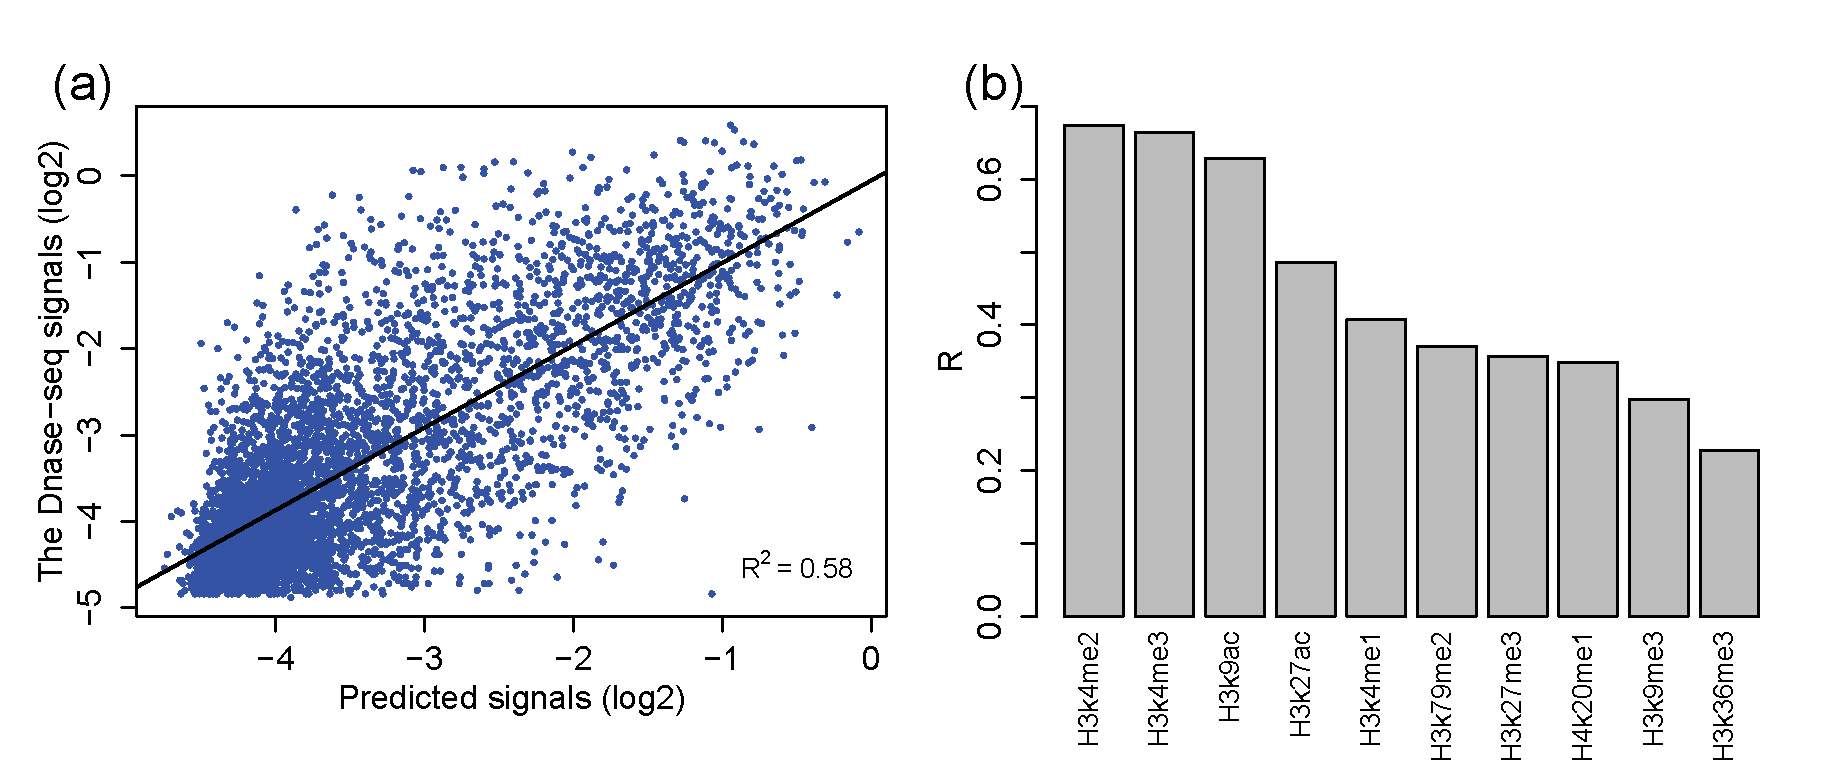
\includegraphics[bb=80bp 0bp 864bp 360bp,scale=0.65]{Figure2}\newpage{}

\textbf{Figure 3.}

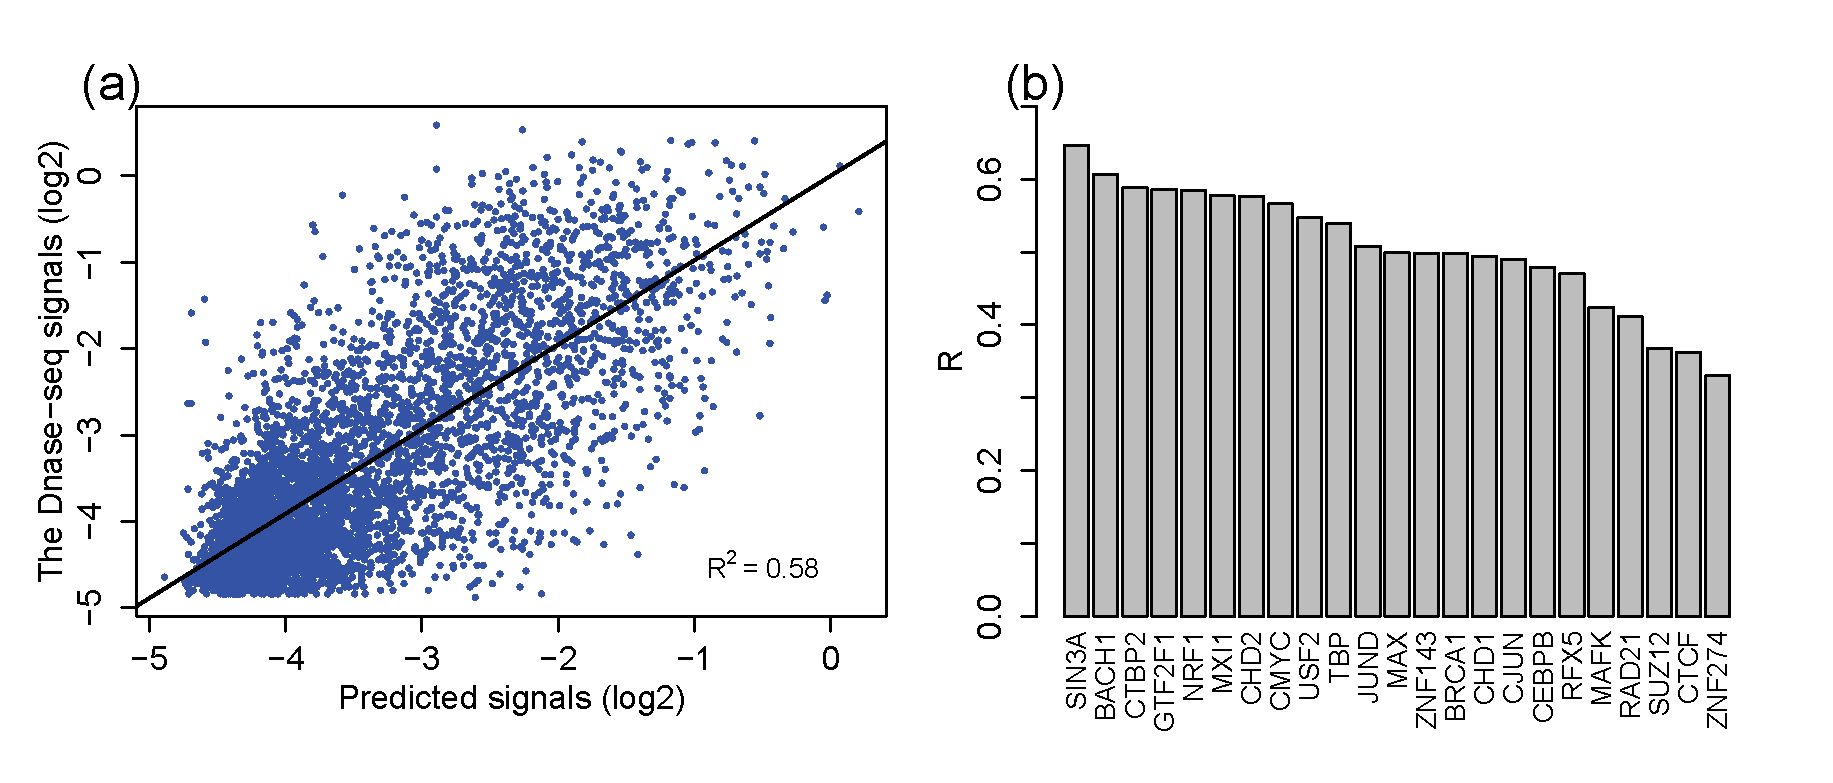
\includegraphics[bb=80bp 0bp 864bp 360bp,scale=0.65]{Figure3}

\newpage{}

\textbf{Figure 4.}

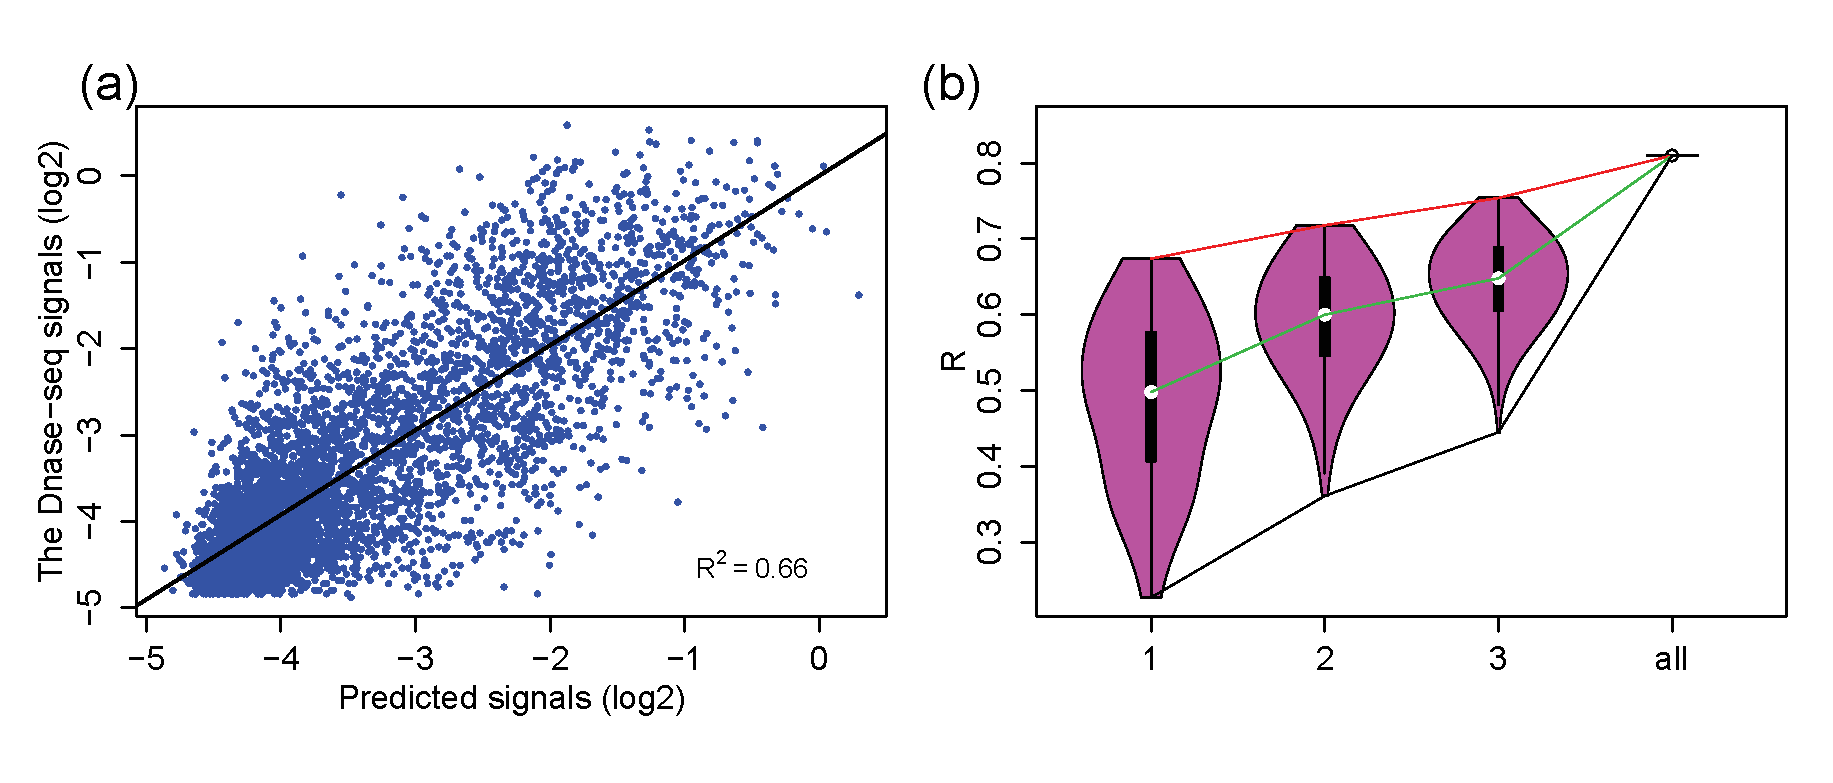
\includegraphics[bb=80bp 0bp 864bp 360bp,scale=0.65]{Figure4}\newpage{}

\textbf{Table 1.}\\


\begin{tabular}{ccccc}
\hline 
Model & SVR & LM & SVR & LM\tabularnewline
 & (max\_signal) & (max\_signal) & (avg\_signal) & (avg\_signal)\tabularnewline
\hline 
HM & 0.76 & 0.69 & 0.70 & 0.56\tabularnewline
TF & 0.76 & 0.63 & 0.69 & 0.53\tabularnewline
HM+TF & 0.81 & 0.73 & 0.75 & 0.61\tabularnewline
\hline 
\end{tabular}
\end{document}
